%% generato automaticamente da tools/build_tex.py --- non modificare
\chapter{Il difetto $\varepsilon$}
\label{cap:teoria}
\quaderno{teoria.dfw}{06 May 2009}{27}

Il quaderno più antico della raccolta — 6 maggio 2009 — e anche il più programmatico. Non contiene un calcolo ma un'idea: che ogni operazione aritmetica, applicata a quantità note in modo imperfetto, restituisca il risultato giusto più un difetto. Il difetto si chiama $\varepsilon$ e le venticinque espressioni che seguono ne inseguono il comportamento: quali operazioni lo lasciano intatto, quali lo amplificano, e in che modo. La sezione finale rivela da dove viene: $\varepsilon$ è la distanza fra $0{,}999\ldots9$ e $1$, cioè il residuo di un troncamento decimale.

\section{Quali operazioni conservano il difetto}

Le prime sette espressioni sono una tavola comparativa. Somma e differenza compaiono senza $\varepsilon$: se i due addendi sono esatti, lo è anche il risultato. Prodotto e quoziente, invece, lo introducono con segni opposti, e le operazioni di ordine superiore lo introducono in forma moltiplicativa. È una classificazione informale ma corretta nella sostanza: le operazioni lineari trasportano l'errore, quelle non lineari lo deformano.

\begin{espr}{1}{User}{}
\[
x + y = k
\]
\end{espr}
La somma non introduce difetto: se $x$ e $y$ sono noti esattamente, $k$ lo è.

\begin{espr}{2}{User}{}
\[
x - y = k
\]
\end{espr}
Lo stesso vale per la differenza. Sono le due operazioni lineari.

\begin{espr}{3}{User}{}
\[
x\, y = k - \varepsilon
\]
\end{espr}
Il prodotto perde $\varepsilon$: il risultato è leggermente inferiore al valore ideale.

\begin{espr}{4}{User}{}
\[
\frac{x}{y} = k + \varepsilon
\]
\end{espr}
Il quoziente lo guadagna, con segno opposto a quello del prodotto: le due operazioni inverse spostano il difetto nelle due direzioni.

\begin{espr}{5}{User}{}
\[
x^{\frac{1}{n}} = x^{\frac{1}{n}}\, p^{\varepsilon}
\]
\end{espr}
L'estrazione di radice non aggiunge un difetto, lo moltiplica: compare come fattore $p^{\varepsilon}$, cioè come un errore relativo.

\begin{espr}{6}{User}{}
\[
x^{2} = x^{2} - \varepsilon
\]
\end{espr}
Elevare al quadrato sottrae $\varepsilon$, coerentemente con la riga $\#3$: il quadrato è un prodotto.

\begin{espr}{7}{User}{}
\[
x = \log_{y}\!\left(y^{x} - \varepsilon\right)
\]
\end{espr}
Il logaritmo è la via di ritorno: recupera $x$ da $y^x$ a patto di scontare il difetto.

\section{La propagazione nelle potenze}

Qui il quaderno si fa preciso. Si prende $x=1/n$ e si calcolano le potenze successive, annotando ogni volta il difetto che le accompagna. Le sei righe sembrano sei casi slegati; in realtà seguono un'unica legge, che non è scritta da nessuna parte nel file ma si ricava confrontandole.

\begin{espr}{8}{User}{}
\[
\left(\frac{1}{n}\right)^{2} = \left(\frac{1}{n}\right)^{2} + 2\, \varepsilon\, \left(\frac{1}{n}\right)
\]
\end{espr}
Primo caso della legge: il quadrato di $1/n$ porta un difetto $2\varepsilon/n$. Si riconosce la derivata: $\mathrm{d}(x^2)=2x\,\mathrm{d}x$.

\begin{espr}{9}{User}{}
\[
\left(\frac{1}{n}\right)^{3} = \left(\frac{1}{n}\right)^{3} + 3\, \varepsilon\, \left(\frac{n + 1}{n^{2}}\right)
\]
\end{espr}
Al cubo il difetto diventa $3\varepsilon(n+1)/n^2$. Il coefficiente $3$ è $\binom{3}{1}$, il termine costante $1$ è $\binom{3}{2}/3$.

\begin{espr}{10}{User}{}
\[
\left(\frac{1}{n}\right)^{4} = \left(\frac{1}{n}\right)^{4} + 4\, \varepsilon\, \left(\frac{n^{2} + \frac{3\, n}{2} + 1}{n^{3}}\right)
\]
\end{espr}
I coefficienti $1,\ 3/2,\ 1$ moltiplicati per $4$ danno $4,\ 6,\ 4$: la quarta riga del triangolo di Tartaglia privata degli estremi.

\begin{espr}{11}{User}{}
\[
\left(\frac{1}{n}\right)^{5} = \left(\frac{1}{n}\right)^{5} + 5\, \varepsilon\, \left(\frac{n^{3} + 2\, n^{2} + 2\, n + 1}{n^{4}}\right)
\]
\end{espr}
Moltiplicati per $5$: $5,\ 10,\ 10,\ 5$. La regola è ormai leggibile a occhio nudo.

\begin{espr}{12}{User}{}
\begin{align*}
& \left(\frac{1}{n}\right)^{6} \\
=\;& \left(\frac{1}{n}\right)^{6} + 6\, \varepsilon\, \left(\frac{n^{4} + \frac{15\, n^{3}}{6} + \frac{10\, n^{2}}{3} + \frac{15\, n}{6} + 1}{n^{5}}\right)
\end{align*}
\end{espr}
Moltiplicati per $6$: $6,\ 15,\ 20,\ 15,\ 6$. La simmetria del polinomio è quella del triangolo binomiale.

\begin{espr}{13}{User}{}
\begin{align*}
& \left(\frac{1}{n}\right)^{7} \\
=\;& \left(\frac{1}{n}\right)^{7} + 7\, \varepsilon\, \left(\frac{n^{5} + 3\, n^{4} + 10\, n^{3} + 5\, n^{2} + 3\, n + 1}{n^{6}}\right)
\end{align*}
\end{espr}
Questa riga rompe la simmetria, e la rottura è rivelatrice. Moltiplicando per $7$ si ottiene $7,\ 21,\ 70,\ 35,\ 21,\ 7$, mentre la legge — e la simmetria delle cinque righe precedenti — richiede $7,\ 21,\ 35,\ 35,\ 21,\ 7$. Il termine in $n^3$ è il doppio di quello che dovrebbe essere: si tratta con ogni probabilità di un errore di battitura ($10$ al posto di $5$ nel numeratore), e lo scarto rispetto alla formula corretta vale esattamente $35\varepsilon/n^3$.


Mettendo $x=1/n$, i difetti annotati nelle espressioni da $\#8$ a $\#12$ sono esattamente $\varepsilon\left[(1+x)^m-1-x^m\right]$, cioè $\varepsilon$ moltiplicato per la parte centrale dello sviluppo binomiale di $(1+x)^m$: spariscono il primo e l'ultimo termine, restano tutti i termini misti. I coefficienti che compaiono nei numeratori sono i binomiali $\binom{m}{1},\binom{m}{2},\dots,\binom{m}{m-1}$, e infatti si leggono a occhio nelle righe $\#10$ e $\#12$: $4,6,4$ e $6,15,20,15,6$.

\section{Una radice doppia è fragile quanto $\sqrt{\varepsilon}$}

Le sei espressioni che seguono contengono l'osservazione più acuta del quaderno, ed è un risultato classico dell'analisi numerica riscoperto per conto proprio. Si parte da un'equazione con radice doppia e si guarda che cosa succede se il termine noto è sbagliato di poco.

\begin{espr}{14}{User}{}
\[
\left(x + 1\right)^{2} = x^{2} + 2\, x + 1 = 0
\]
\end{espr}
Un'equazione con radice doppia in $x=-1$: il caso peggiore per la stabilità.

\begin{espr}{15}{User}{}
\[
x = -1 - \sqrt{2\, \varepsilon} \;\lor\; x = -1 + \sqrt{2\, \varepsilon}
\]
\end{espr}
Perturbando il termine noto di $2\varepsilon$, la radice doppia si sdoppia in due radici distanti $\sqrt{2\varepsilon}$ dal valore nominale.

\begin{espr}{16}{User}{}
\[
x - x = 2\, \sqrt{2\, \varepsilon}
\]
\end{espr}
La distanza fra le due radici perturbate. La scrittura $x-x$ è volutamente paradossale: sono due valori che dovrebbero coincidere e non coincidono.

\begin{espr}{17}{User}{}
\[
\left(x - 1\right)^{2} = x^{2} - 2\, x + 1 = 0
\]
\end{espr}
Lo stesso esperimento sulla radice doppia in $x=+1$.

\begin{espr}{18}{User}{}
\[
x = 1 - \sqrt{2\, \varepsilon} \;\lor\; x = \sqrt{2\, \varepsilon} + 1
\]
\end{espr}
Le due radici perturbate, simmetriche rispetto a $1$.

\begin{espr}{19}{User}{}
\[
x - x = 2\, \sqrt{2\, \varepsilon}
\]
\end{espr}
La separazione è la stessa: dipende solo dall'entità della perturbazione, non da dove si trova la radice.

\begin{figure}[htbp]
  \centering
  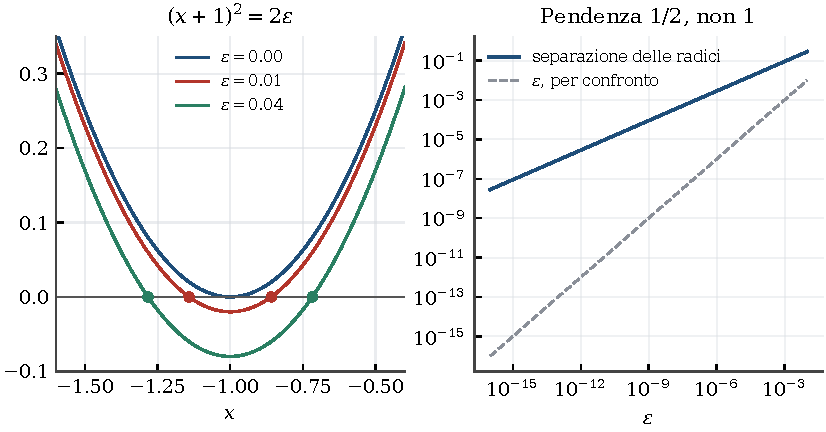
\includegraphics[width=0.86\linewidth]{../figures/teoria_radice_doppia.pdf}
  \caption{Una perturbazione di ampiezza $2\varepsilon$ sul termine noto separa le due radici di $(x+1)^2=0$ di una quantità proporzionale a $\sqrt{\varepsilon}$, non a $\varepsilon$. In scala doppiamente logaritmica la pendenza $1/2$ è la firma della radice doppia.}
  \label{fig:teoria_radice_doppia}
\end{figure}

Il punto è nell'ordine di grandezza. Se il polinomio $(x+1)^2$ viene perturbato di una quantità $2\varepsilon$, le due radici non si spostano di $\varepsilon$: si separano di $2\sqrt{2\varepsilon}$. Con $\varepsilon=10^{-16}$, cioè la precisione di un numero in doppia precisione, la separazione è dell'ordine di $10^{-8}$: otto cifre perse di colpo. È la ragione per cui le radici multiple sono il caso peggiore per qualunque risolutore numerico, ed è notevole vederla isolata così, in quattro righe.

\section{Da dove viene $\varepsilon$}

L'ultima sezione scopre le carte. Il difetto non è un'astrazione: è quello che resta quando si tronca uno sviluppo decimale. Le due espressioni $\#20$ e $\#21$ costruiscono i due protagonisti — un numero fatto di mille cifre $9$ e il prodotto delle potenze successive di $1/10$ — e le successive chiedono quando i due si corrispondano esattamente.

\begin{espr}{20}{User}{}
\[
\mathrm{U} = \sum_{n=0}^{999} 9 \cdot 10^{n}
\]
\end{espr}
Un numero di mille cifre, tutte $9$. La variabile ha un nome non alfabetico, conservato qui come compariva nel file.

\begin{espr}{21}{User}{}
\[
\varepsilon = \prod_{n=1}^{999} \left(\frac{1}{10}\right)^{n}
\]
\end{espr}
Il prodotto vale $10^{-499500}$: un numero minuscolo, il candidato naturale al ruolo di $\varepsilon$.

\begin{espr}{22}{User}{}
\[
\prod_{n=1}^{x} \left(\frac{1}{10}\right)^{n} = \frac{1}{\sum_{n=0}^{x} 9 \cdot 10^{n}}
\]
\end{espr}
L'equazione centrale del quaderno. A sinistra $10^{-x(x+1)/2}$, a destra $1/(10^{x+1}-1)$.

\begin{espr}{23}{Simp(Solve(\#22,x))}{}
\begin{align*}
& 10^{x\, \left(x + 1\right)} - 10^{2\, \left(x + 1\right)} + 2^{x + 2} \cdot 5^{x + 1} = 1 \\[3pt]
\lor\quad & x = \infty + \frac{3\, \pi\, \mathrm{i}}{\ln\!\left(10\right)} \\[3pt]
\lor\quad & x = \infty - \frac{2\, \pi\, \mathrm{i}}{\ln\!\left(10\right)} \\[3pt]
\lor\quad & x = \infty + \frac{2\, \pi\, \mathrm{i}}{\ln\!\left(10\right)} \\[3pt]
\lor\quad & x = \infty - \frac{\pi\, \mathrm{i}}{\ln\!\left(10\right)} \\[3pt]
\lor\quad & x = \infty + \frac{\pi\, \mathrm{i}}{\ln\!\left(10\right)} \\[3pt]
\lor\quad & x = \infty
\end{align*}
\end{espr}
La risposta di Derive: una condizione algebrica più una famiglia di soluzioni all'infinito, generate dalla periodicità immaginaria dell'esponenziale complesso ($2\pi\mathrm{i}/\ln 10$ è il periodo di $10^{z}$).

\begin{espr}{24}{User}{}
\[
10^{x\, \left(x + 1\right)} - 10^{2\, \left(x + 1\right)} + 2^{x + 2} \cdot 5^{x + 1} = 1
\]
\end{espr}
La condizione algebrica isolata. Si ottiene elevando al quadrato $10^{x(x+1)/2}=10^{x+1}-1$; il termine $2^{x+2}5^{x+1}$ non è altro che $2\cdot 10^{x+1}$.

\begin{espr}{25}{Simp(Solve(\#24,x))}{}
\[
x = 1.999710103
\]
\end{espr}
La soluzione numerica: $x$ manca il valore intero $2$ per tre parti su diecimila.

\begin{espr}{26}{Solve(\#22,x)}{}
\[
\operatorname{NSolve}\!\left(\prod_{n=1}^{x} \left(\frac{1}{10}\right)^{n} = \frac{1}{\sum_{n=0}^{x} 9 \cdot 10^{n}},\; x\right)
\]
\end{espr}
La stessa domanda posta al risolutore numerico anziché a quello simbolico.

\begin{espr}{27}{Simp(Solve(\#22,x))}{}
\[
x = 10
\]
\end{espr}
Il valore restituito è $x=10$, che non soddisfa l'equazione: è un artefatto della ricerca numerica, che si è fermata su un punto in cui i due membri sono entrambi enormi e la loro differenza relativa è sotto la soglia di tolleranza. Vale la pena conservarlo come promemoria: un risolutore numerico risponde sempre, anche quando non dovrebbe.


La risposta è il cuore del quaderno. L'equazione $\#22$ si riscrive come $10^{x(x+1)/2}=10^{x+1}-1$: a sinistra una potenza di dieci, a destra una potenza di dieci meno uno. Per $x=2$ i due membri valgono $1000$ e $999$. Non sono uguali — ma lo sono a meno di una parte su mille, e la soluzione numerica $\#25$ lo conferma: $x=1{,}999710\ldots$ invece di $2$. Quel $-1$ che impedisce l'uguaglianza è $\varepsilon$. Tutto il quaderno gira intorno a lui.

\section*{In sintesi}
\addcontentsline{toc}{section}{In sintesi}

Il quaderno non dimostra nulla in senso stretto e non ne ha l'intenzione. Fissa un'intuizione — l'errore come oggetto con leggi proprie — e la mette alla prova su tre fronti: la propagazione nelle potenze, dove trova per via sperimentale i coefficienti binomiali; la sensibilità delle radici multiple, dove ritrova il comportamento $\sqrt{\varepsilon}$ che rende quel caso patologico; e l'origine decimale del difetto, dove $\varepsilon$ si rivela essere il $-1$ di $10^{k}-1$. Delle sei righe sulla propagazione, cinque combaciano con la legge generale e una contiene un refuso: anche questo, in un quaderno sull'errore, ha il suo posto.

